\chapter{Example Analysis}
%can also add tractography for common areas such as the cingulum, etc here.
%fix formatting
The section presents the analysis of a set of DWI using the stochastic tractography system.  In addition to sampling all possible fibers from a seed region, the system can also sample only fibers which are conditioned to pass through a second labeled region.  Each analysis is performed with and without a white matter map to demonstrate differences in the results under these two conditions.  Without the white matter map, tracts are allowed to pass through regions of grey matter, which may not have fiber bundles.  Using the white matter map constrains the tracts to pass through only white matter known to have fiber bundles.  Finally results obtained using stochastic tractography results are compared with those obtained under streamlining tractography.
\begin{figure}
\label{fig:labelmap}
  \center
	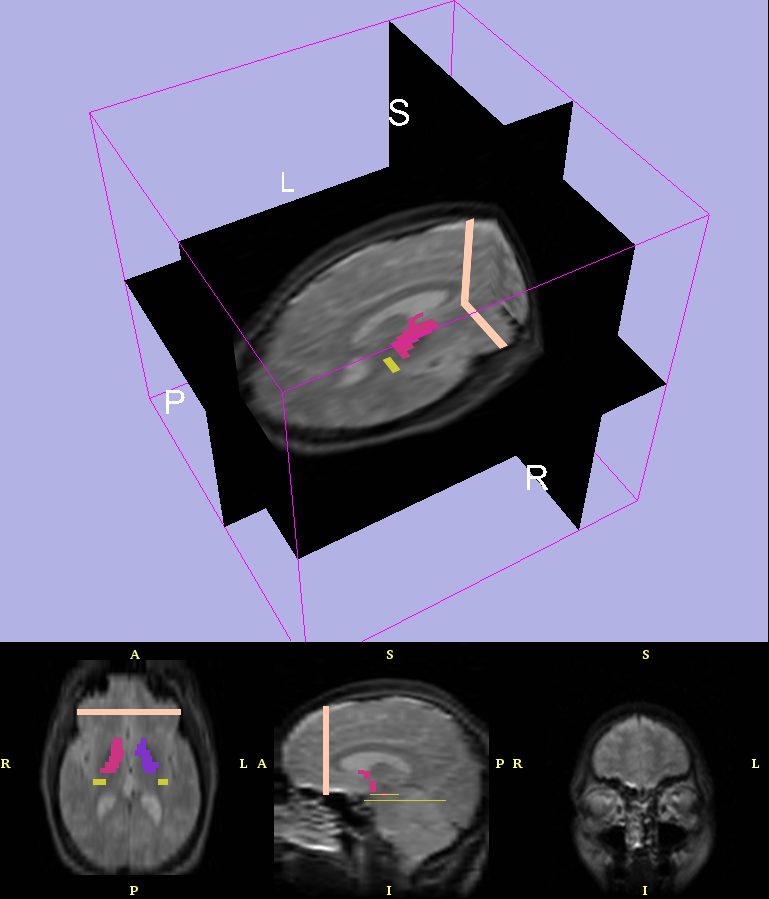
\includegraphics[width=0.5\linewidth]{slicer-0001}
	\caption{The non-diffusion weighted b0 image with superimposed right internal capsule and frontal lobe ROI's.}
\end{figure}
The DWI data set was obtained using 6 gradient directions and one b0 image obtained in the absence of diffusion weighted gradients.  The voxels occupy 0.86mm x 0.86mm x 5mm sized cells. The right internal capsule was segmented by an expert by using a fractional anisotropy criteria.  The right internal capsule segmentation is considered the first region of interest (ROI).  A second region of interest(ROI) is placed anterior or towards the front of the brain, in the frontal lobe.  Figure \ref{fig:labelmap} displays the ROI's superimposed on the non-diffusion weighted b0 image of the DTI set.

In the results below, tractography was started in the right internal capsule ROI.  The stochastic tractography system attempted to sample 100 tracts from every voxel in the internal capsule.  The actual number of samples collected may actually be less due to the use of a white matter map, which may exclude portions of the internal capsule ROI, or by rejecting tracts which do not pass through a second ROI.  Without using the white matter map, the tract was terminated when it left the brain or when it reached a maximum length of 500 mm.  From the front, or anterior, of the brain to the rear, or posterior, measures about 185 mm so a 500 mm maximum tract length should be long to enough to generate all anatomically plausible tracts.  When using a white matter map, tracts can only pass through regions of white matter and are terminated when they leave white matter.  As a result, seed points must be in grey matter cannot be used to initiate tractography.
%tell how the white matter was segmented
%talk about how the brain was segmented using BET

%obtain the parameters for the data set
\section{Single ROI}
In these results all possible tracts were sampled which originated from the right internal capsule ROI.

\begin{figure} 
  \label{fig:singlecmaps}
  \subfigure[Without white matter map]{
    \label{fig:singlecmaps:a}
	  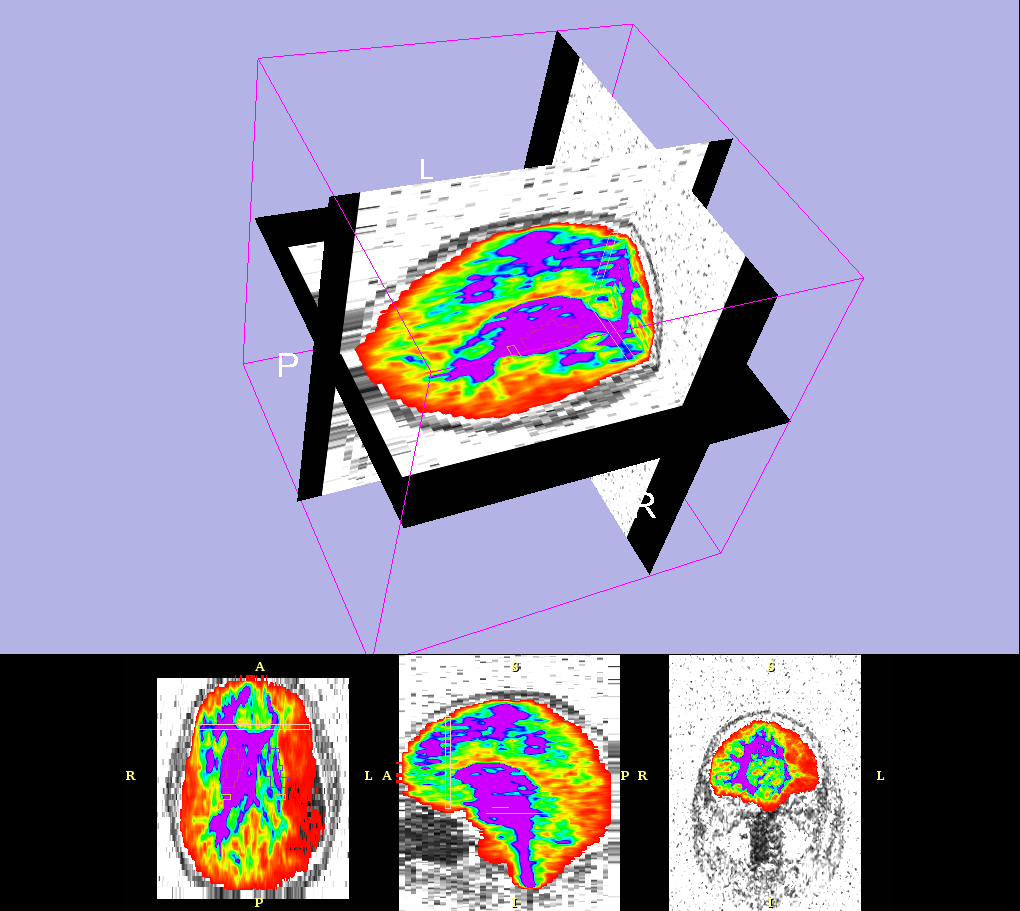
\includegraphics[width=0.5\linewidth]{slicer-0022}
	}
	\subfigure[With white matter map]{
	  \label{fig:singlecmaps:b}
	  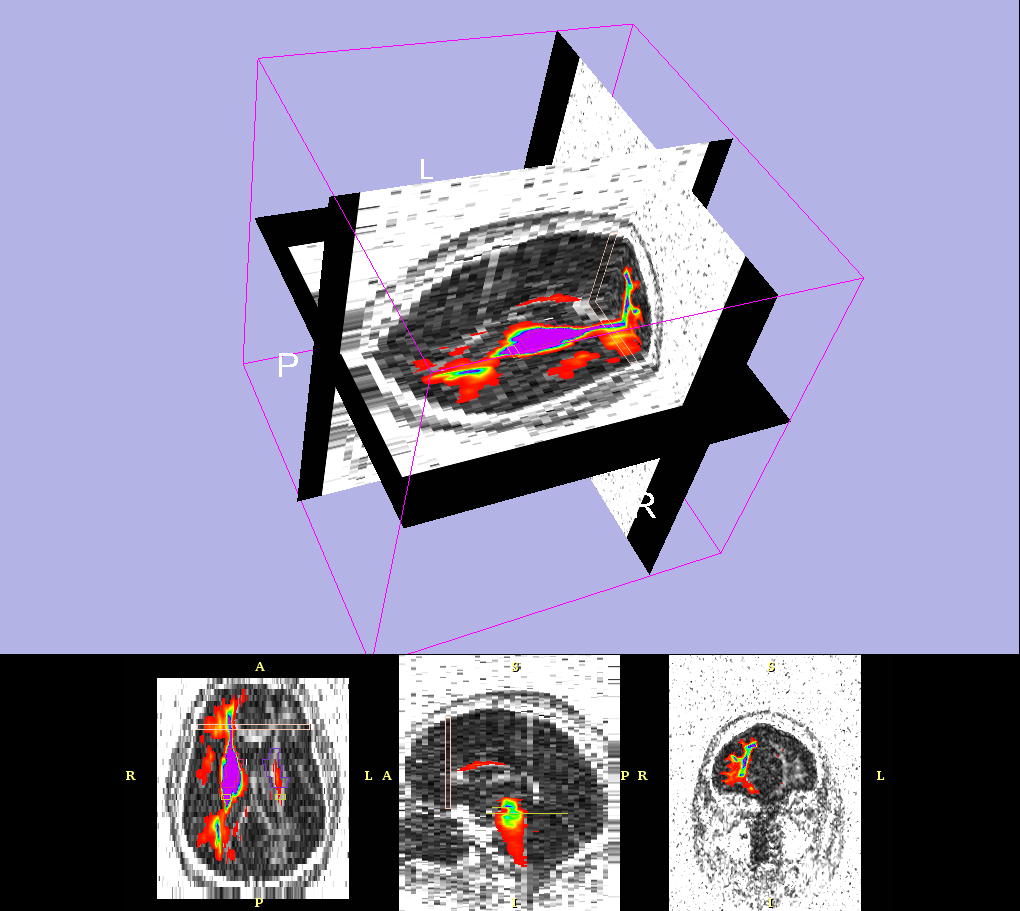
\includegraphics[width=0.5\linewidth]{slicer-0020}
	}
	\caption{Connectivity maps generated using stochastic tractography overlaid on a fractional anisotropy image of the data.  The seed region is the right internal capsule.  Colors indicate the number of tracts originating from the seed region which pass through that voxel.}
\end{figure}

Figure \ref{fig:singlecmaps} presents connectivity maps generated using the stochastic tractography system.  The color of each voxel indicates the number of tracts which pass through that voxel.  Since seeding was initiated in the internal capsule, it appears highly connected to itself in the connectivity map.  Notice the strong connectivity of some voxels in the frontal lobe using stochastic tractography with and without the white matter map.  Without the white matter map \ref{fig:singlecmaps:a} a few sampled tracts cross from the right hemisphere into the left hemisphere of the brain, probably through the highly anisotropic corpus collosum.  The number of these crossover fibers are greatly reduced when the white matter map used and the resultant spatial distribution of the fibers is more concentrated.  Additionally, the number of sampled tracts when using the white matter map is reduced because the right internal capsule ROI may include some grey matter which cannot produce any tract samples.

\begin{figure}
  \label{fig:singleFAhistograms}
  \subfigure[Without white matter map]{
    \label{fig:singleFAhistograms:a}
	  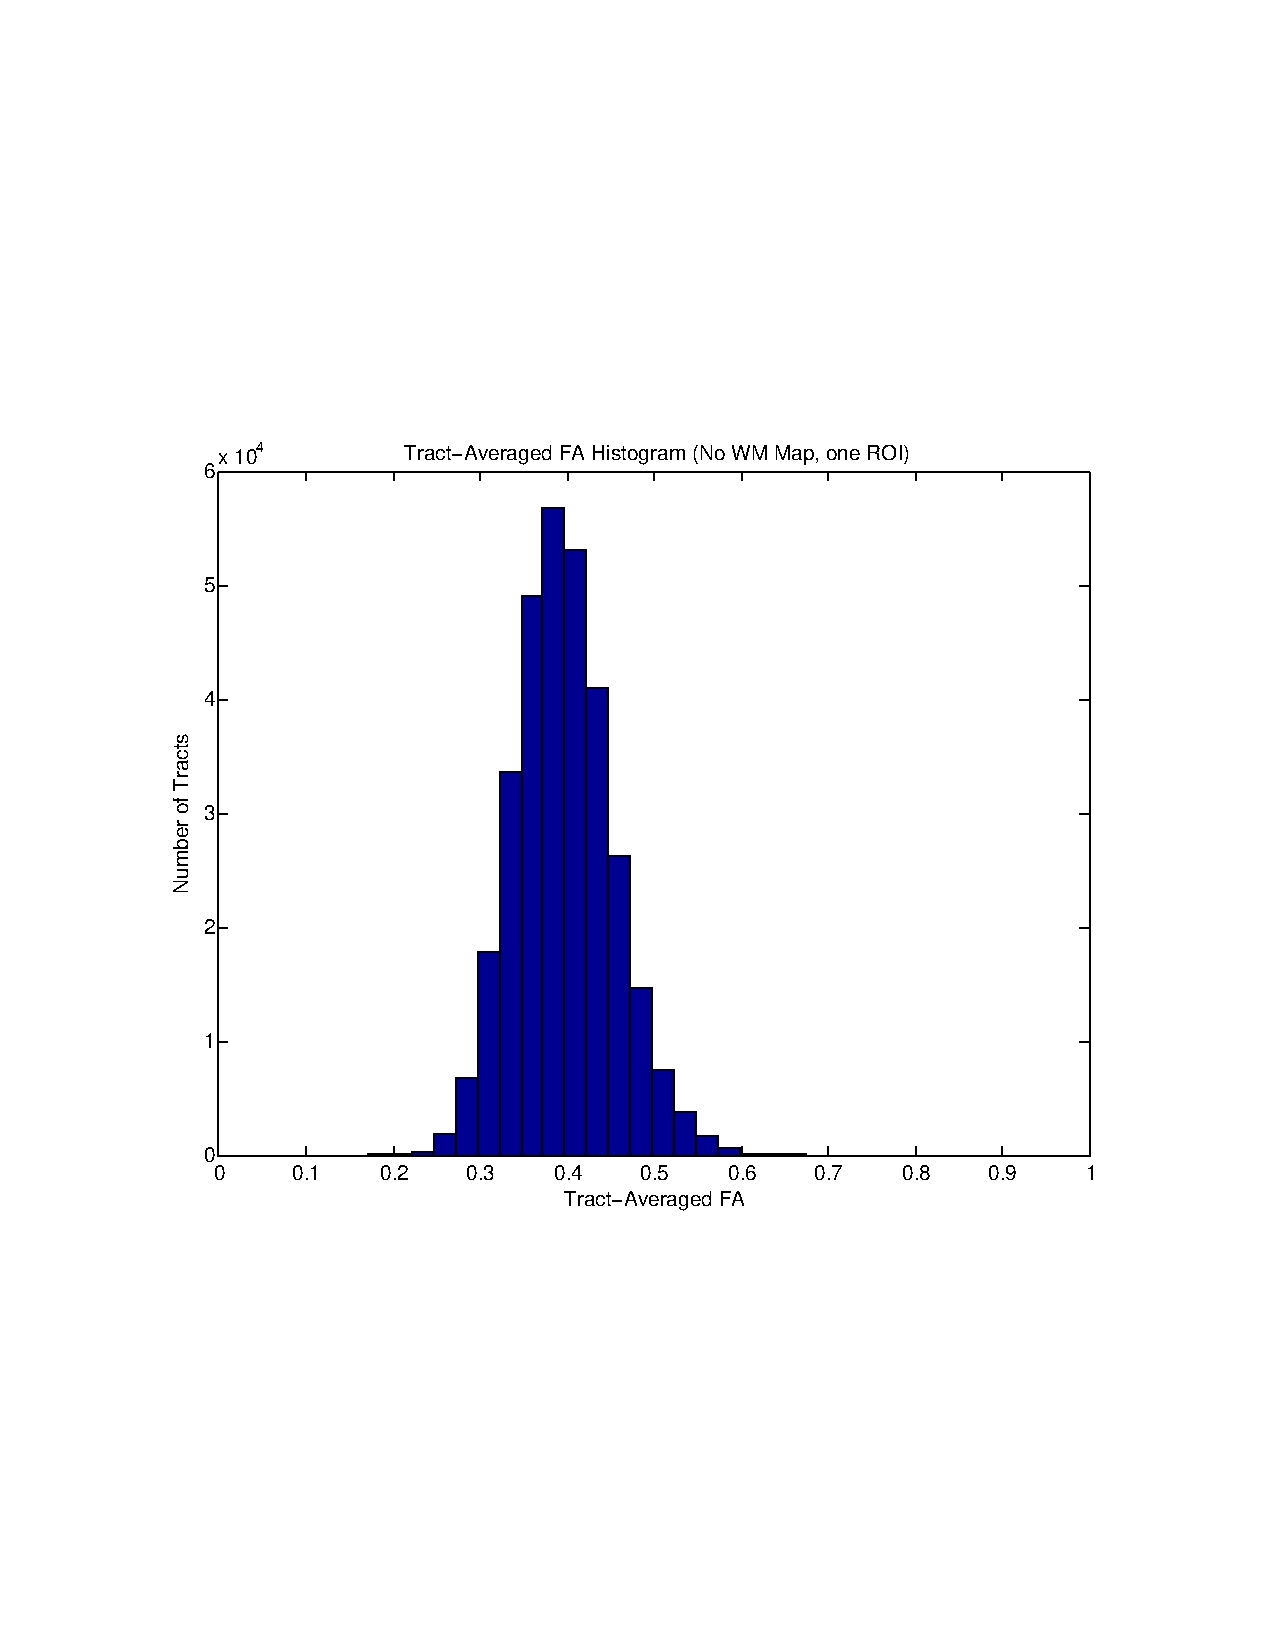
\includegraphics[trim = 20mm 70mm 20mm 70mm, clip, width=0.5\linewidth]
	    {hist_FA_nomask_single}
	}
	\subfigure[with white matter map]{
	  \label{fig:singleFAhistograms:b}
	  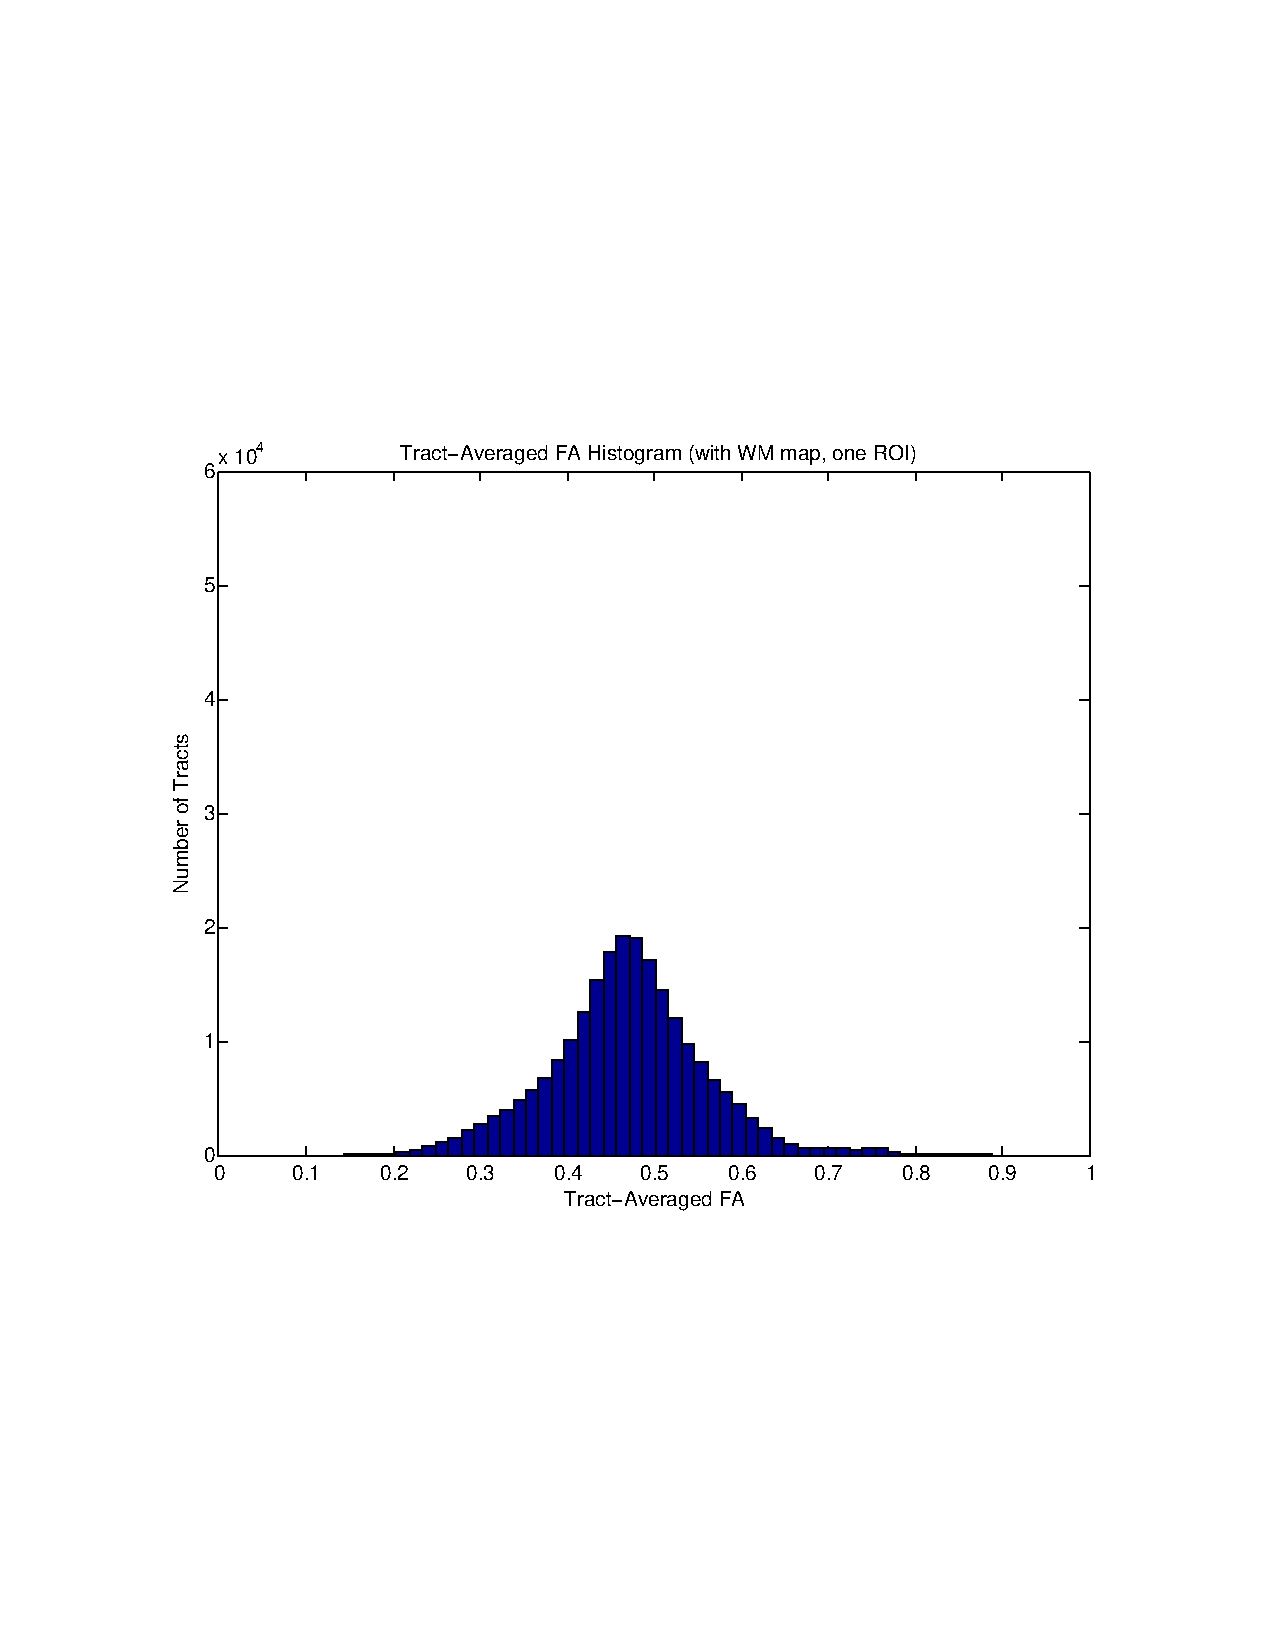
\includegraphics[trim = 20mm 70mm 20mm 70mm, clip, width=0.5\linewidth]
	    {hist_FA_mask_single}
	}
	\caption{Histogram showing distribution of tract-averaged fractional anisotropy for tracts which originate in the right internal capsule.}
\end{figure}

We can also study statistics on individual sampled tracts.  The distribution of tract-averaged fractional anisotropy is graphed in figure \ref{fig:singleFAhistograms}.  Notice that using the white matter map predictably increases the mean of the distribution (Figure \ref{fig:singleFAhistograms:a}), since the sampled tracts no longer pass through gray matter which has low anisotropy.  Additionally, the number of sampled tracts also decreases when using the white matter map because some of the voxels in the right internal capsule ROI were identified as grey matter.

\begin{figure}
  \label{fig:singelengthhistograms}
  \subfigure[Without white matter map]{
    \label{fig:singlelengthhistograms:a}
	  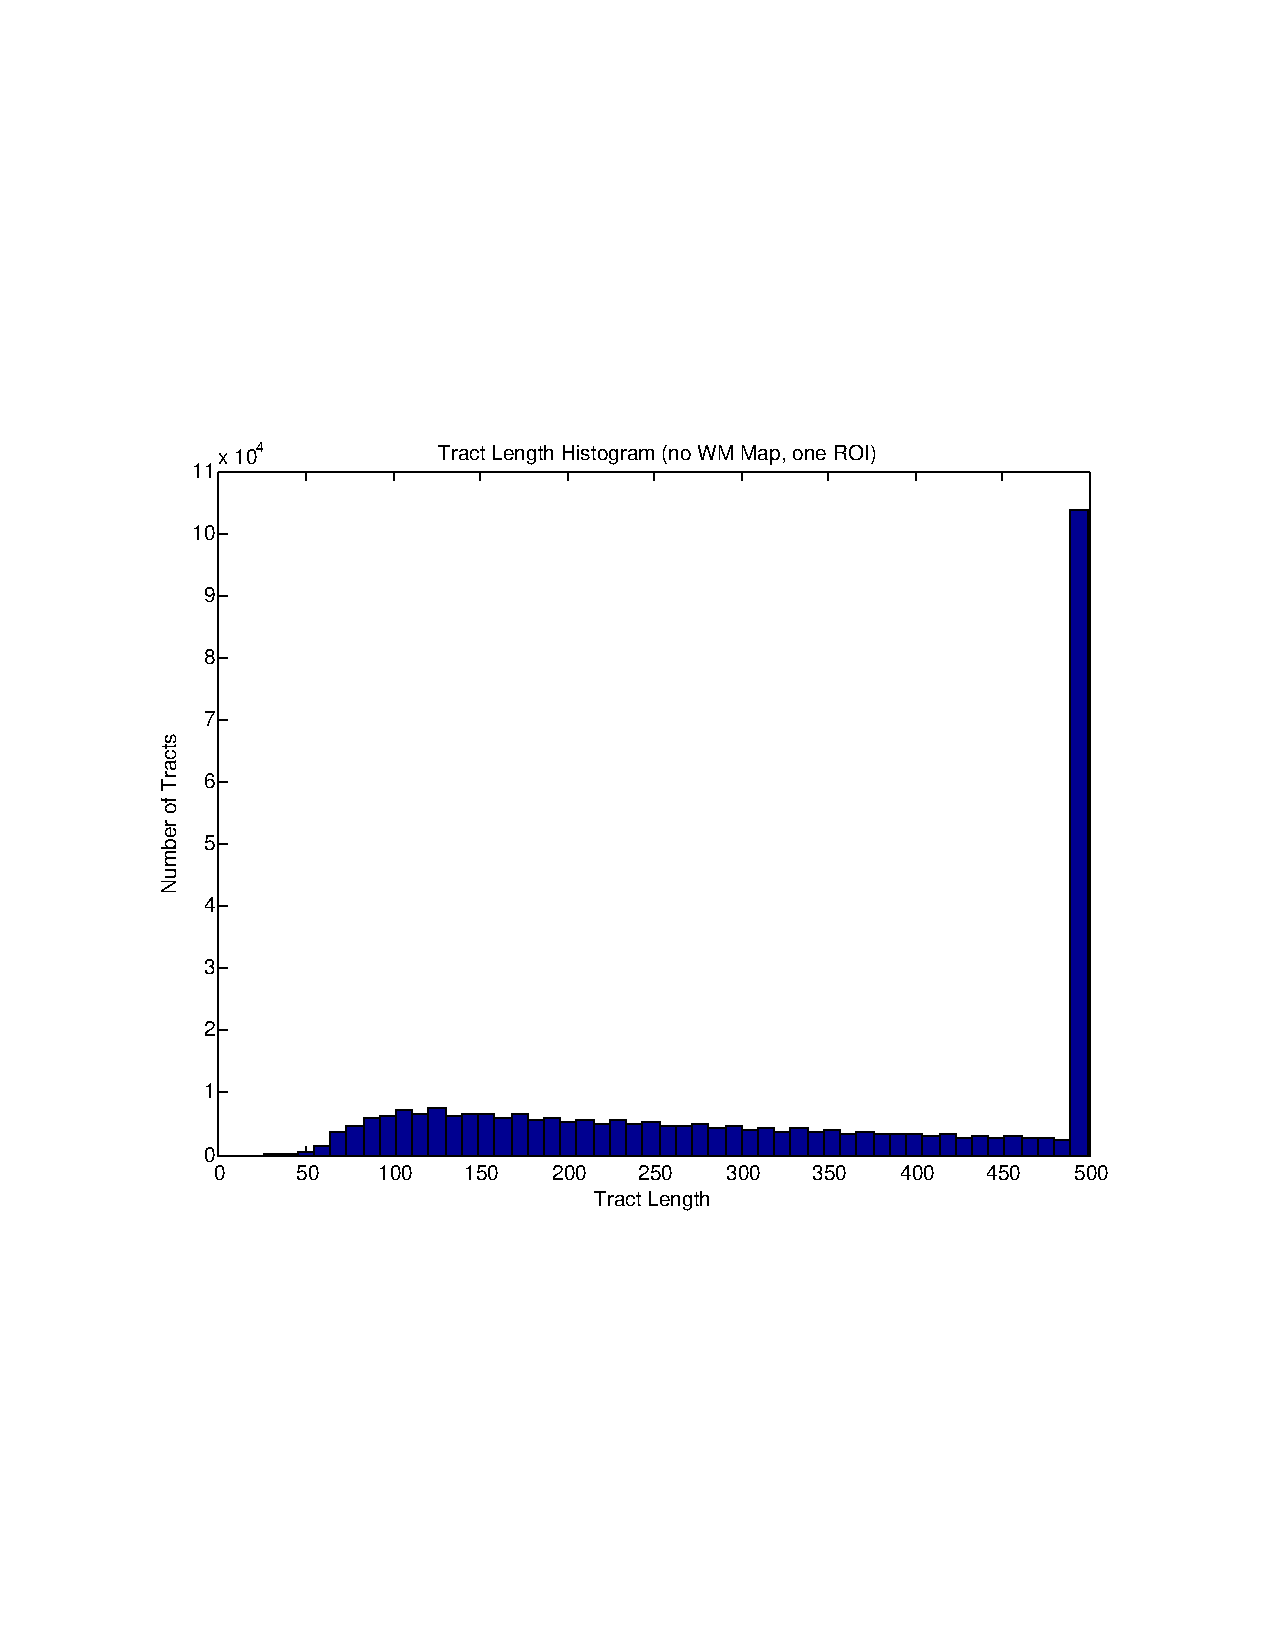
\includegraphics[trim = 20mm 70mm 20mm 70mm, clip, width=0.5\linewidth]
	    {hist_length_nomask_single}
	}
	\subfigure[With white matter map]{
	  \label{fig:singlelengthhistograms:b}
	  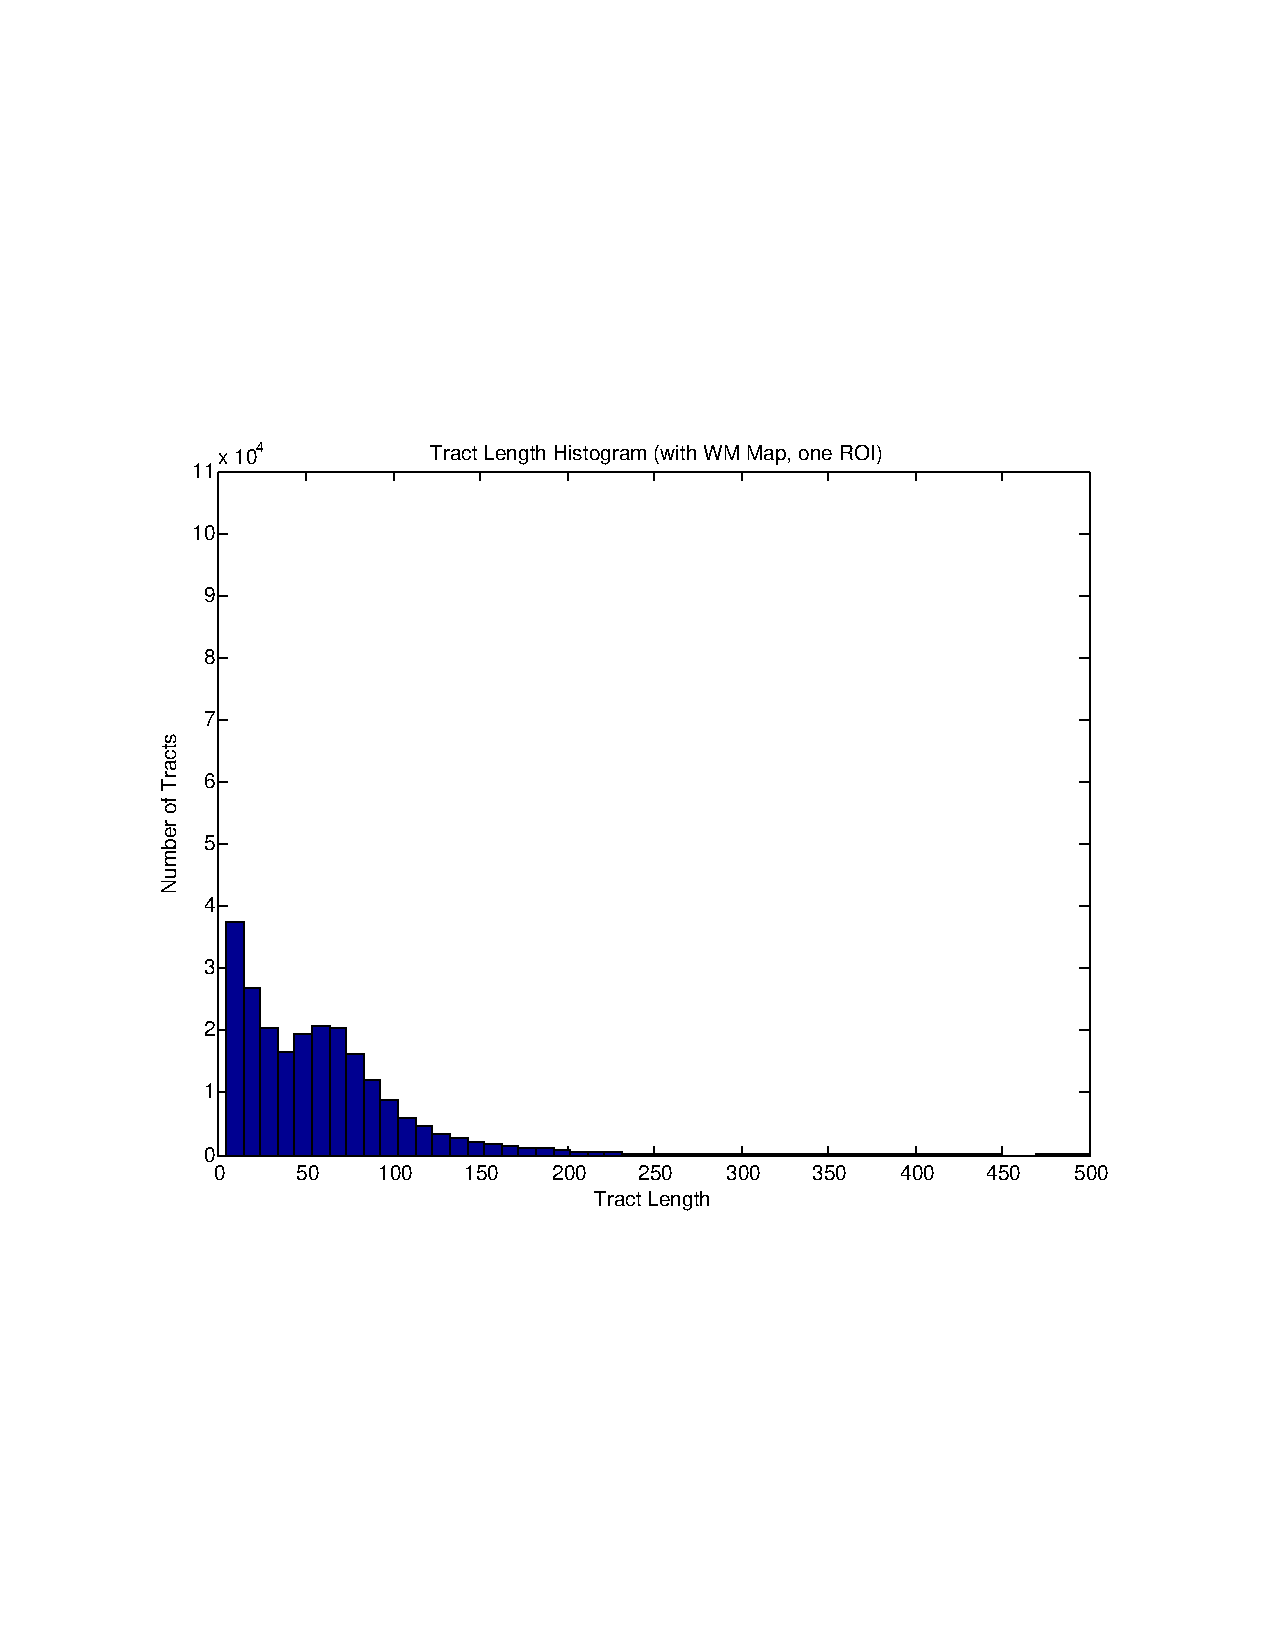
\includegraphics[trim = 20mm 70mm 20mm 70mm, clip, width=0.5\linewidth]
	    {hist_length_mask_single}
	}
	\caption{Histogram showing distribution of fiber lengths for sampled frontal lobe tracts.}
\end{figure}

Figure \ref{fig:singelengthhistograms} plots the distribution of lengths on the sampled tracts.  Without the white matter map many fibers reach the arbitrary maximum tract limit of 500 (Figure \ref{fig:singlelengthhistograms:a}, providing little information about the actual distribution of tract lenghts.  With the white matter posterior probability map, few sampled tracts reach 500mm and the distribution of tract lengths may be more representative of the true distribution.


\section{Two ROIs}

The stochastic tractography system can optionally reject all sampled tracts which do not pass through a second ROI.  This method isolates fiber bundles which connect two ROI.  
\begin{figure} \label{fig:twocmaps}
  \subfigure[Without white matter map]{
    \label{fig:twocmaps:a}
	  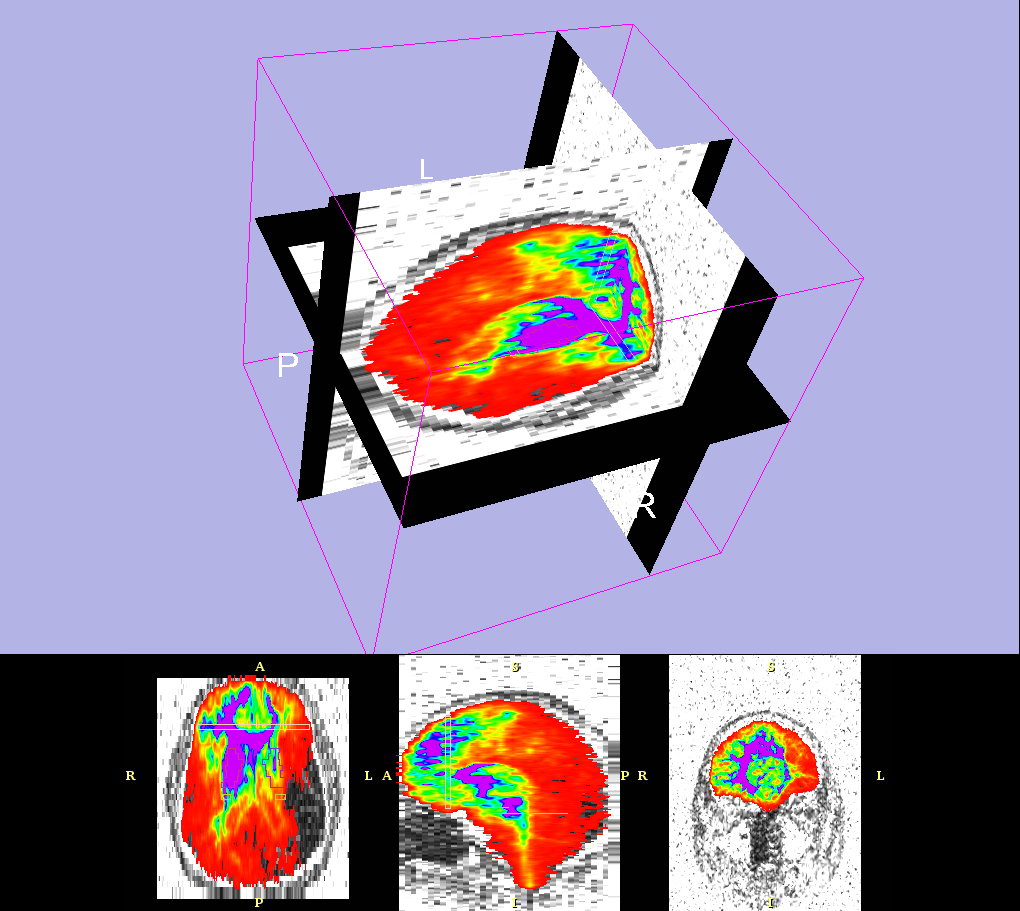
\includegraphics[width=0.5\linewidth]{slicer-0021}
  }
  \subfigure[With white matter map]{
    \label{fig:twocmaps:b}
	  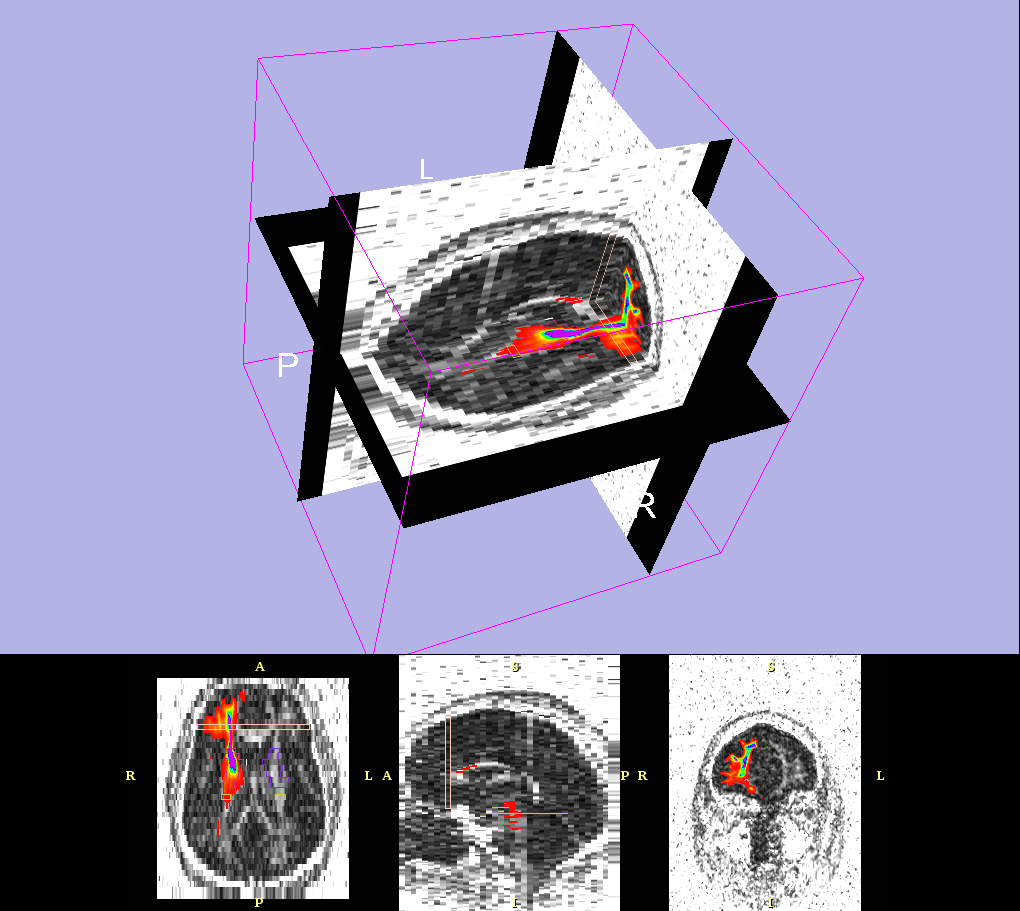
\includegraphics[width=0.5\linewidth]{slicer-0019}
	}
	\caption{Connectivity map overlaid on a fractional anisotropy image showing the probability that a voxel is connected to the internal capsule by a fiber which passes through a second ROI in the frontal lobe.}
\end{figure}

The connectivity maps in Figure \ref{fig:twocmaps} show the probability that a voxel is connected to the right internal capsule by a fiber originating in the right internal capsule which passes through the second ROI located in the frontal lobe.  Unsurprisingly, regions in the frontal lobe are much more likely to be connected via these fibers than anywhere else in the brain.

\begin{figure} \label{fig:twoFAhistograms}
  \subfigure[Without white matter map]{
    \label{fig:twoFAhistograms:a}
	  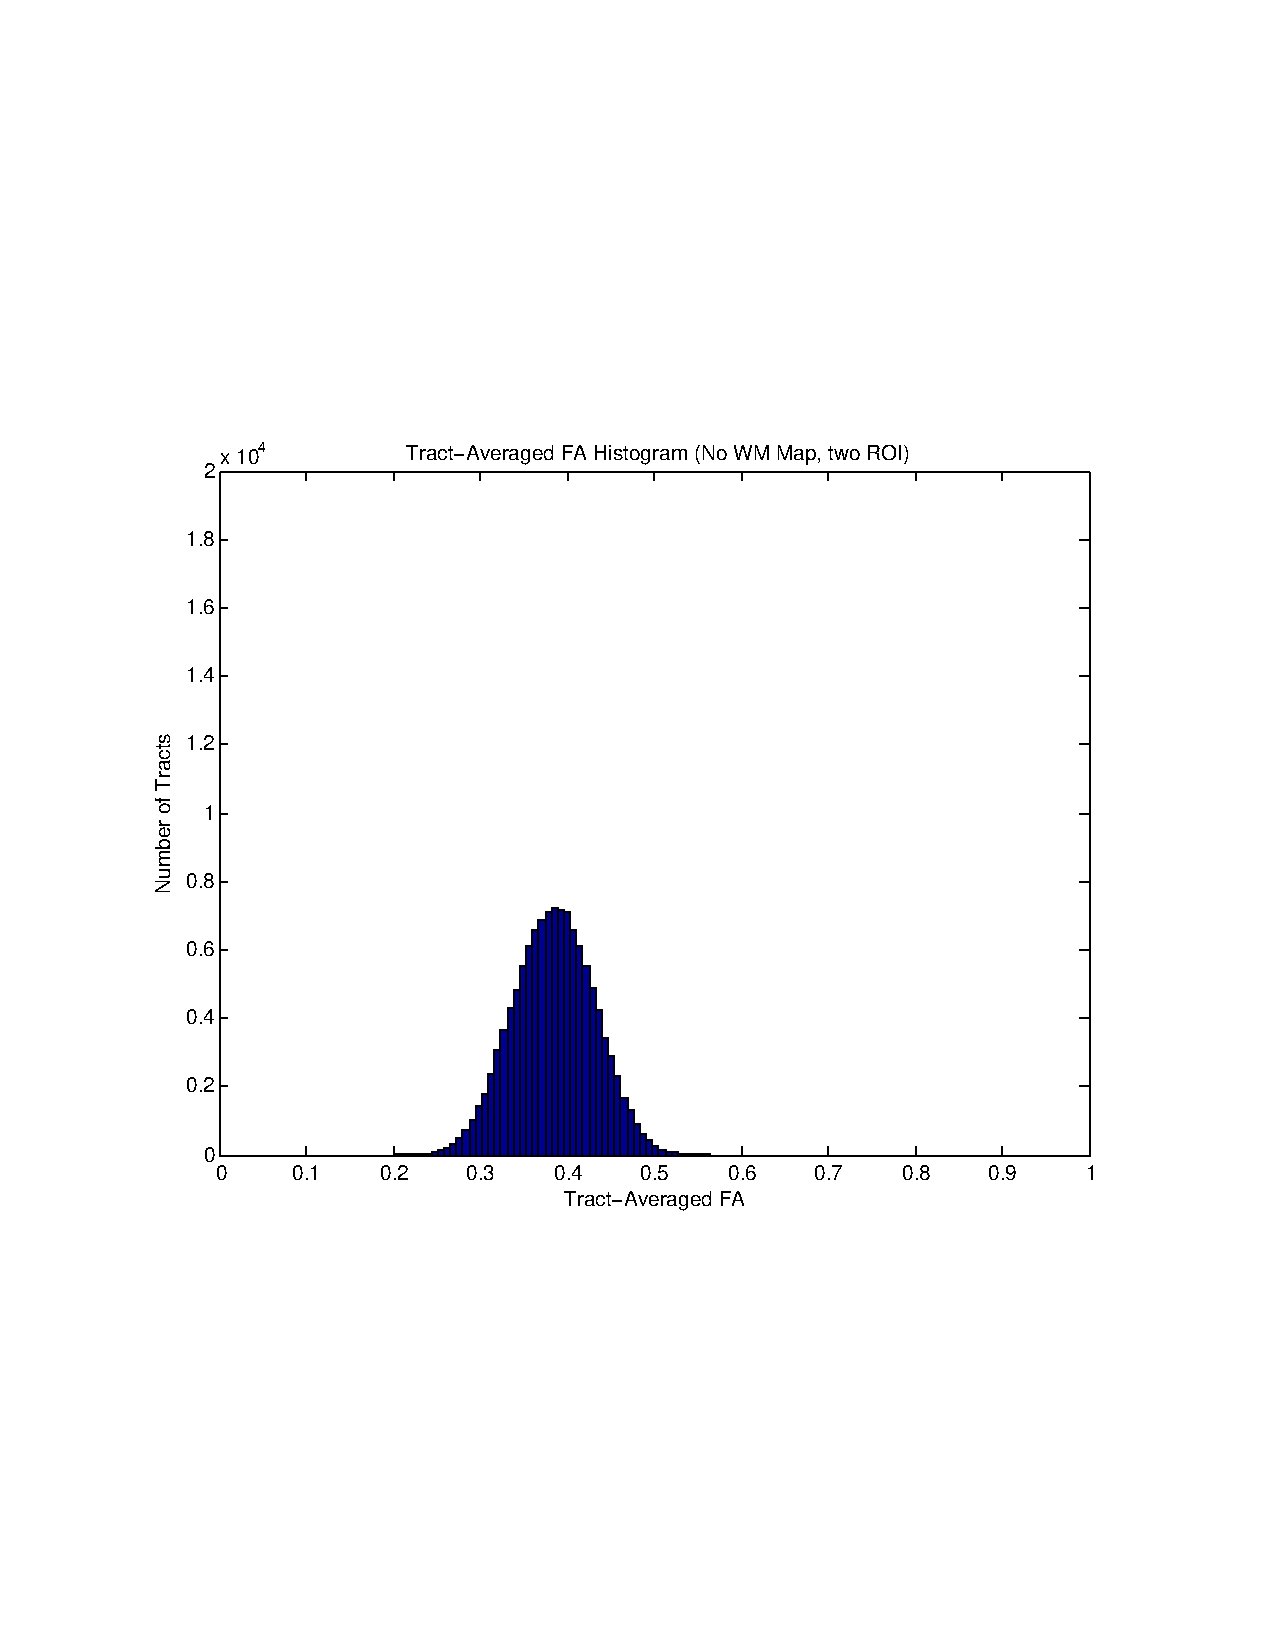
\includegraphics[trim = 20mm 70mm 20mm 70mm, clip, width=0.5\linewidth]
	    {hist_FA_nomask_two}
  }
  \subfigure[With white matter map]{
    \label{fig:twoFAhistograms:b}
	  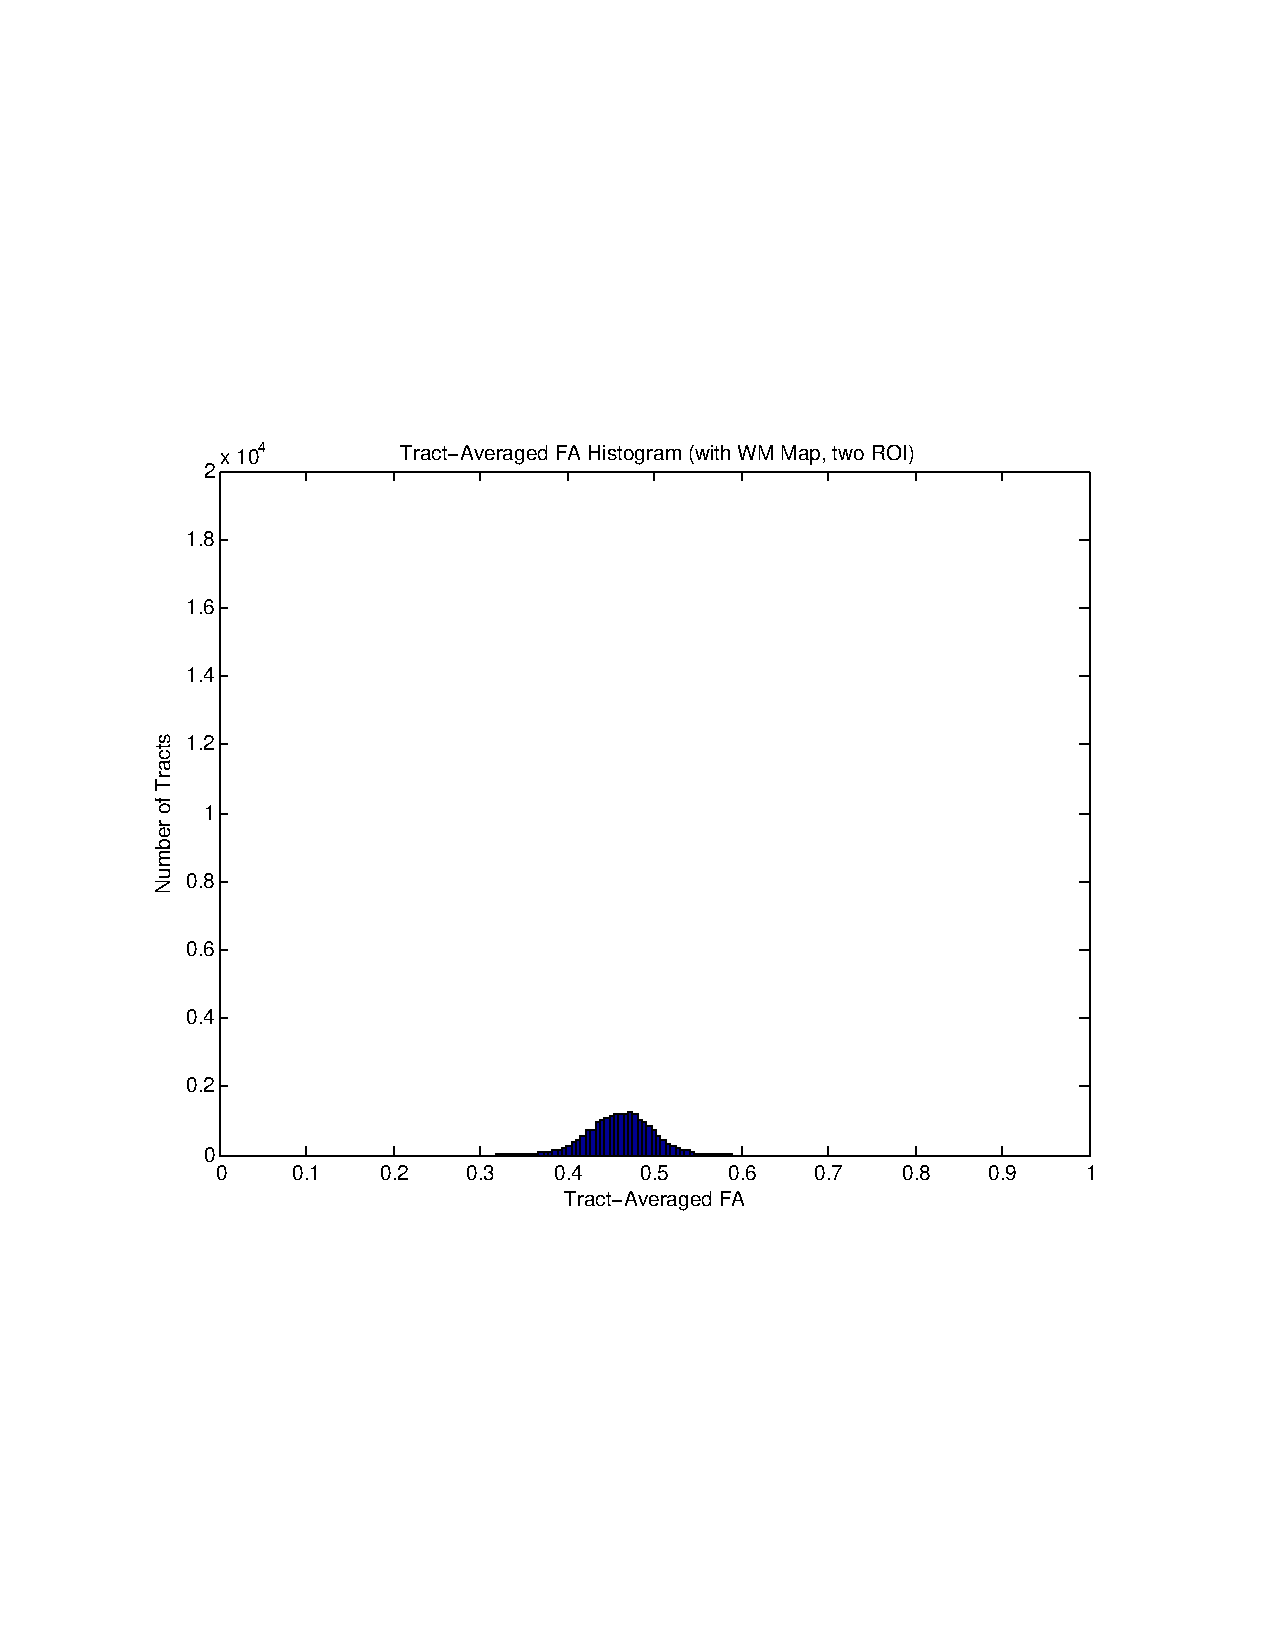
\includegraphics[trim = 20mm 70mm 20mm 70mm, clip, width=0.5\linewidth]
	    {hist_FA_mask_two}
	}
	\caption{A histogram of tract-averaged fractional anisotropy for fibers which originate in the right internal capsule and pass through an ROI in the frontal lobe.}
\end{figure}

Although 100 tract samples were attempted by the algorithm, only a fraction pass through the second ROI.  Thus the histograms in figures \ref{fig:twoFAhistograms} and \ref{fig:twolengthhistograms} contain fewer total tracts than those in figures \ref{fig:singleFAhistograms} and \ref{fig:singelengthhistograms}.  Notice that using the white matter map again increases the mean of the tract-averaged fractional anisotropy distribution (Figure \ref{fig:twoFAhistograms:b}) by preventing tracts from passing through low anisotropy grey matter.

\begin{figure} \label{fig:twolengthhistograms}
  \subfigure[Without white matter map]{
    \label{fig:twolengthhistograms:a}
	  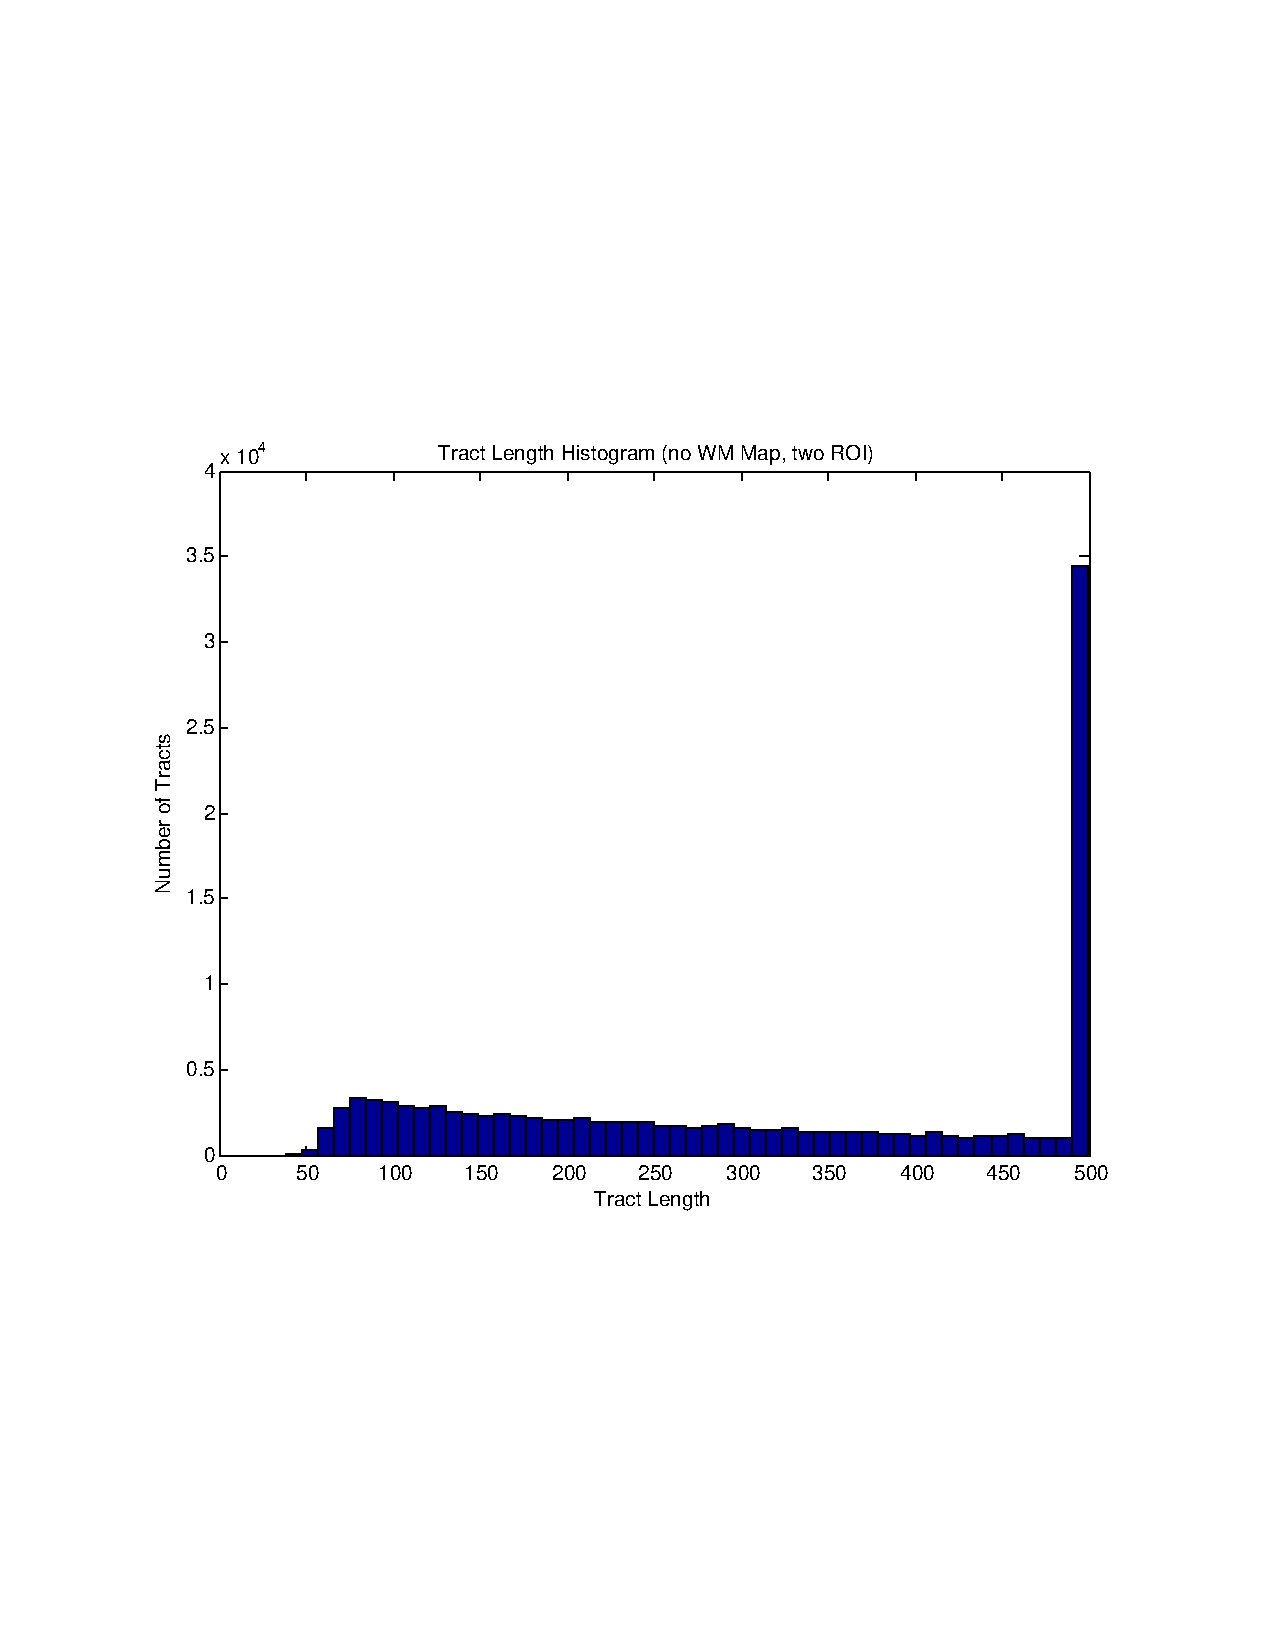
\includegraphics[trim = 20mm 70mm 20mm 70mm, clip, width=0.5\linewidth]
	    {hist_length_nomask_two}
	}
	\subfigure[With white matter map]{
	  \label{fig:twolengthhistograms:b}
	  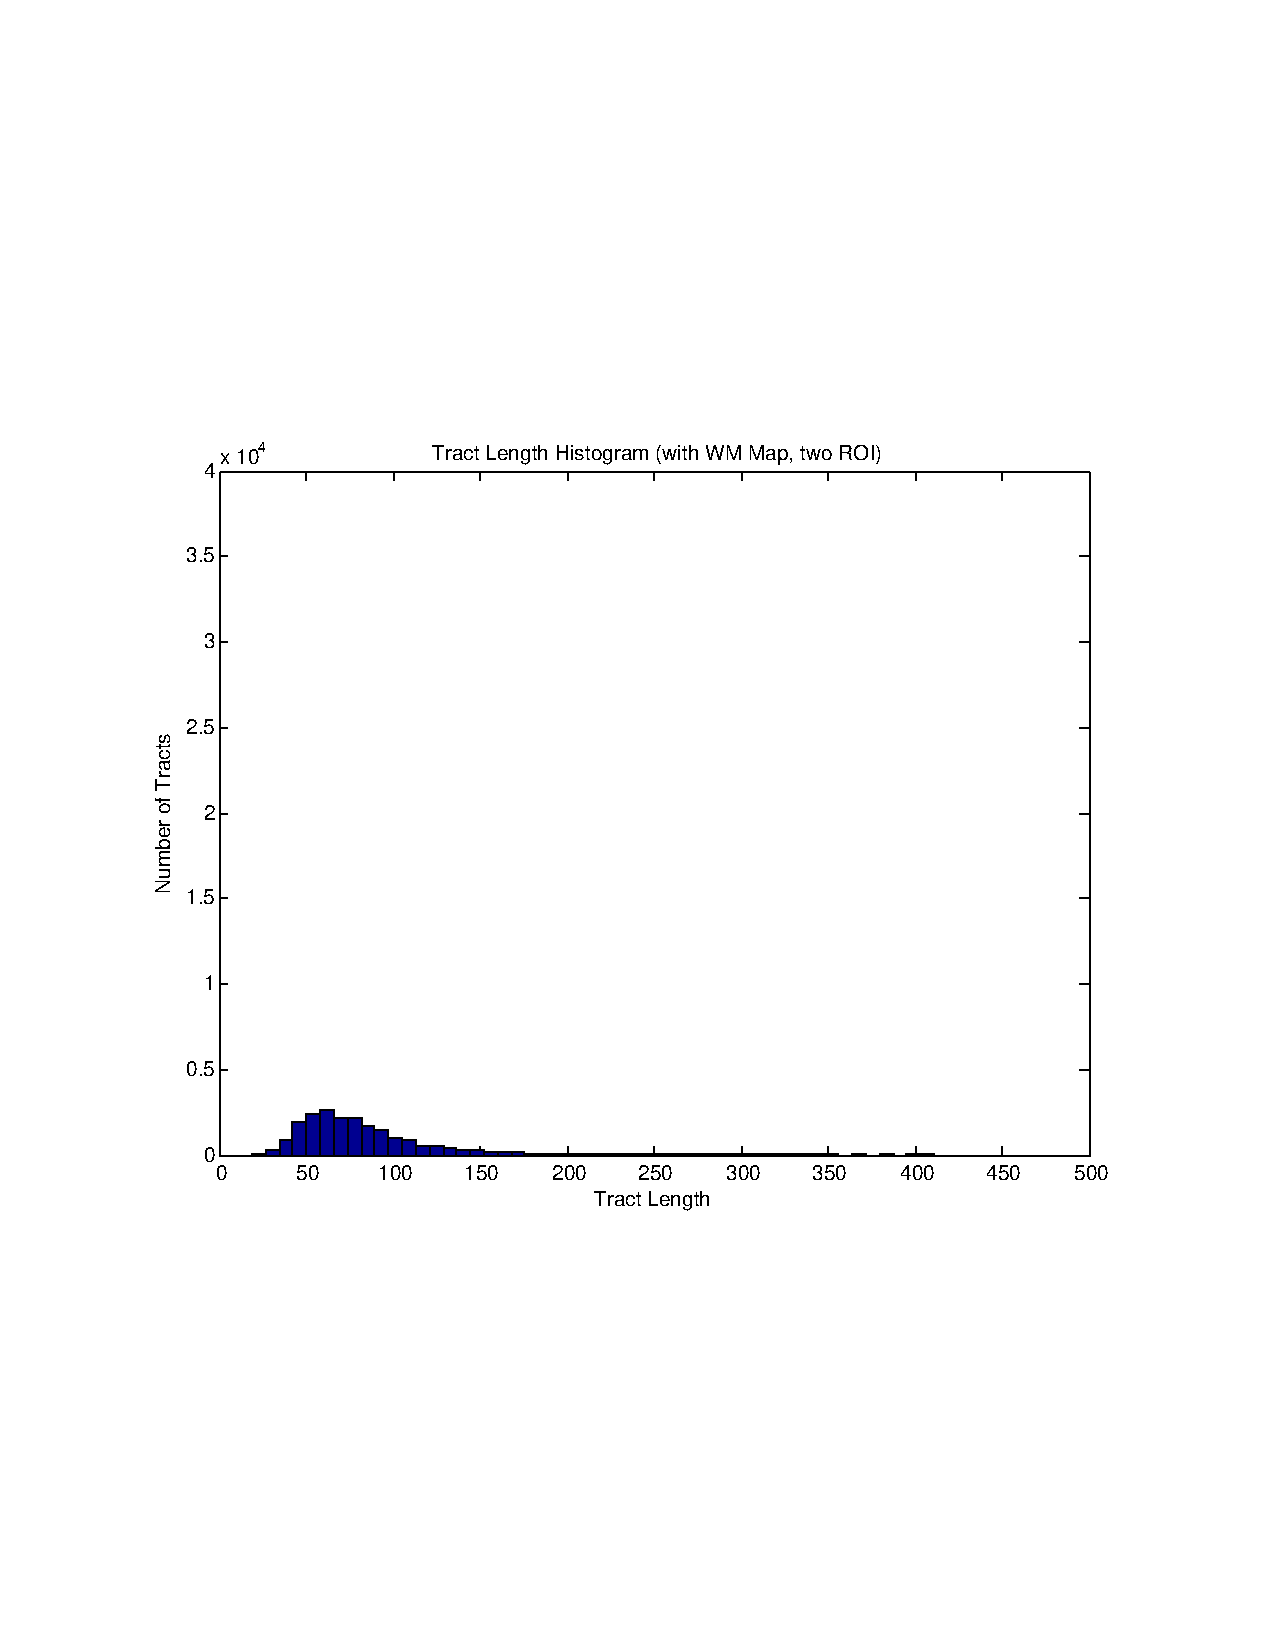
\includegraphics[trim = 20mm 70mm 20mm 70mm, clip, width=0.5\linewidth]
	    {hist_length_mask_two}
  }
	\caption{A histogram of lengths for sampled fibers which start in the right internal capsule and pass through an ROI in the frontal lobe. }
\end{figure}

Figure \ref{fig:twolengthhistograms} demonstrates that using the white matter map provides more meaningful distributions of length than tracking without using one.

\section{Comparison with streamlining tractography}
In this section, streamlining tractography and stochastic tractography are run on the same data using the same ROI's.  The streamlining tractography results are generated using the streamline tractography method in 3D Slicer.  The streamline method used every voxel inside the segmented internal capsule as a seed region.  The generated streamline tracts were only accepted if they passed through the second ROI in the frontal lobe.  Tracking was terminated in the streamline method when the current voxel's anisotropy fell below a minimum threshold.  The stochastic tractography results are the same as in the previous section's two ROI analysis depicted in figures \ref{fig:twoFAhistograms} and \ref{fig:twolengthhistograms}.

\begin{figure} \label{fig:streamlinecomp}
  \subfigure[Streamlining results]{
    \label{fig:streamlinecomp:a}
	  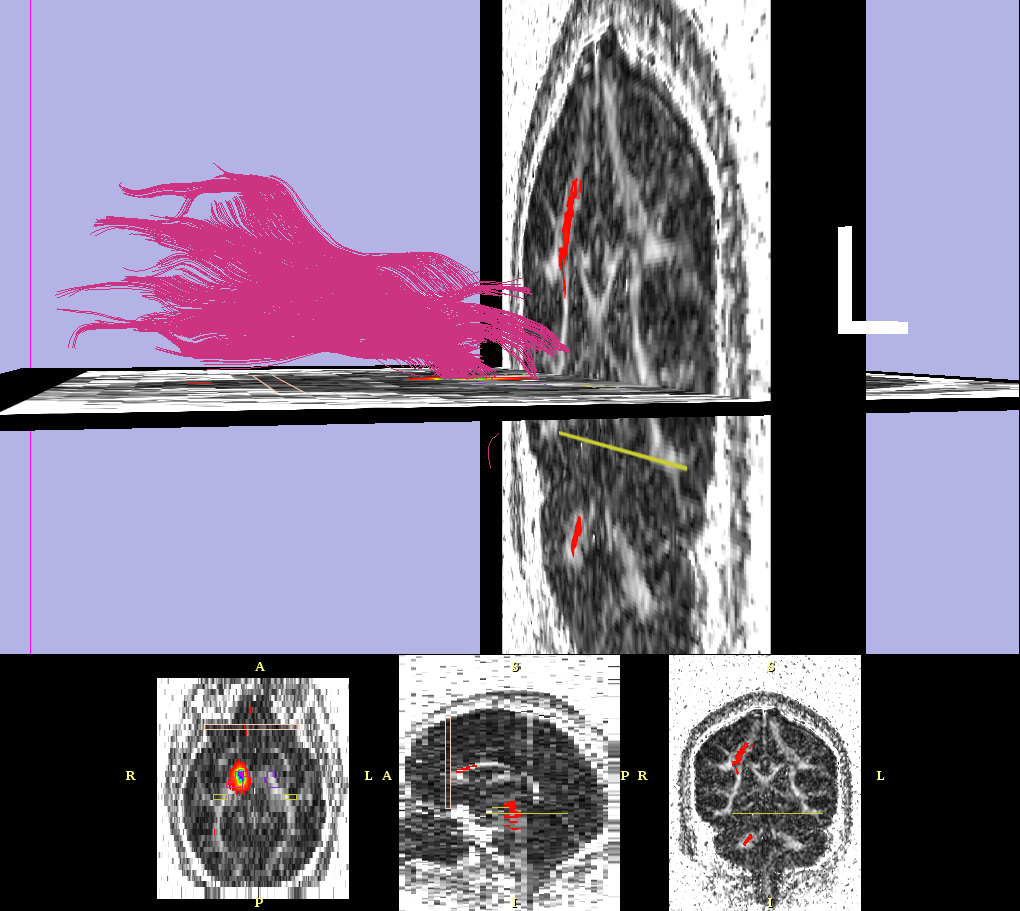
\includegraphics[width=0.5\linewidth]
	    {slicer-0016}
	  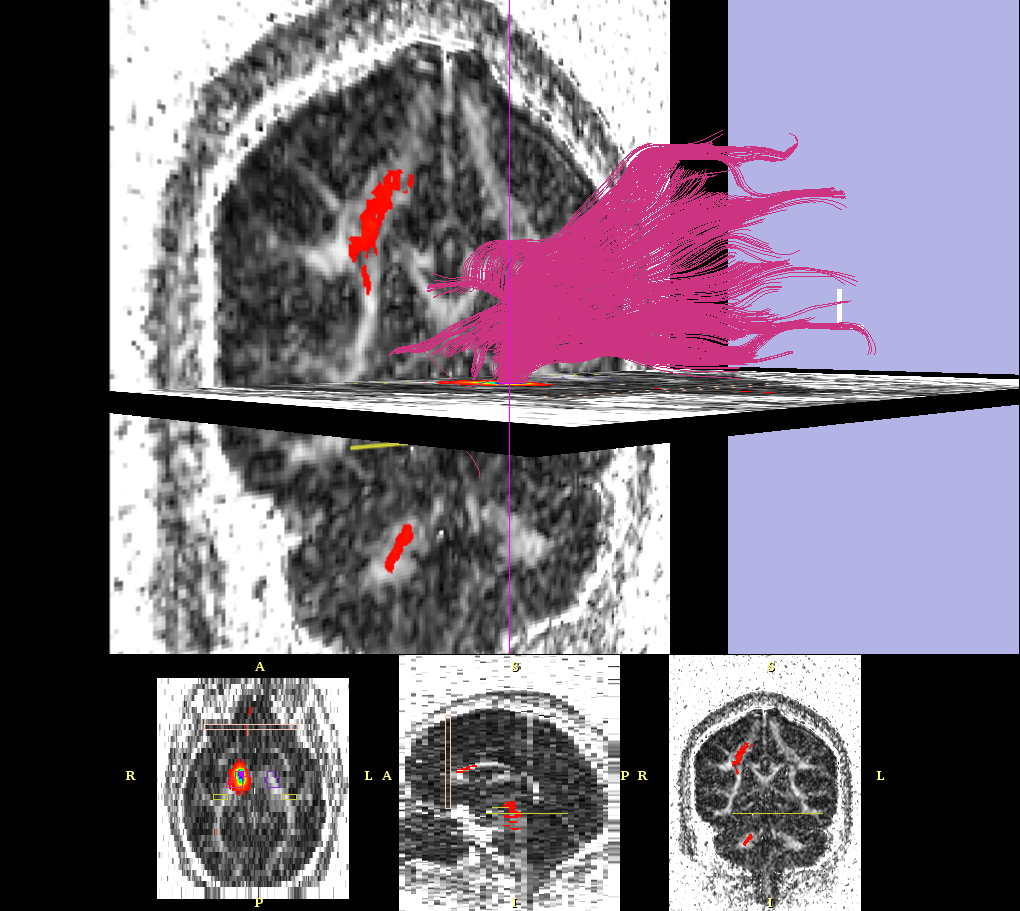
\includegraphics[width=0.5\linewidth]
	    {slicer-0018}
  }
  \subfigure[Streamlining results with volume rendered connectivity map]{
    \label{fig:streamlinecomp:b}
	  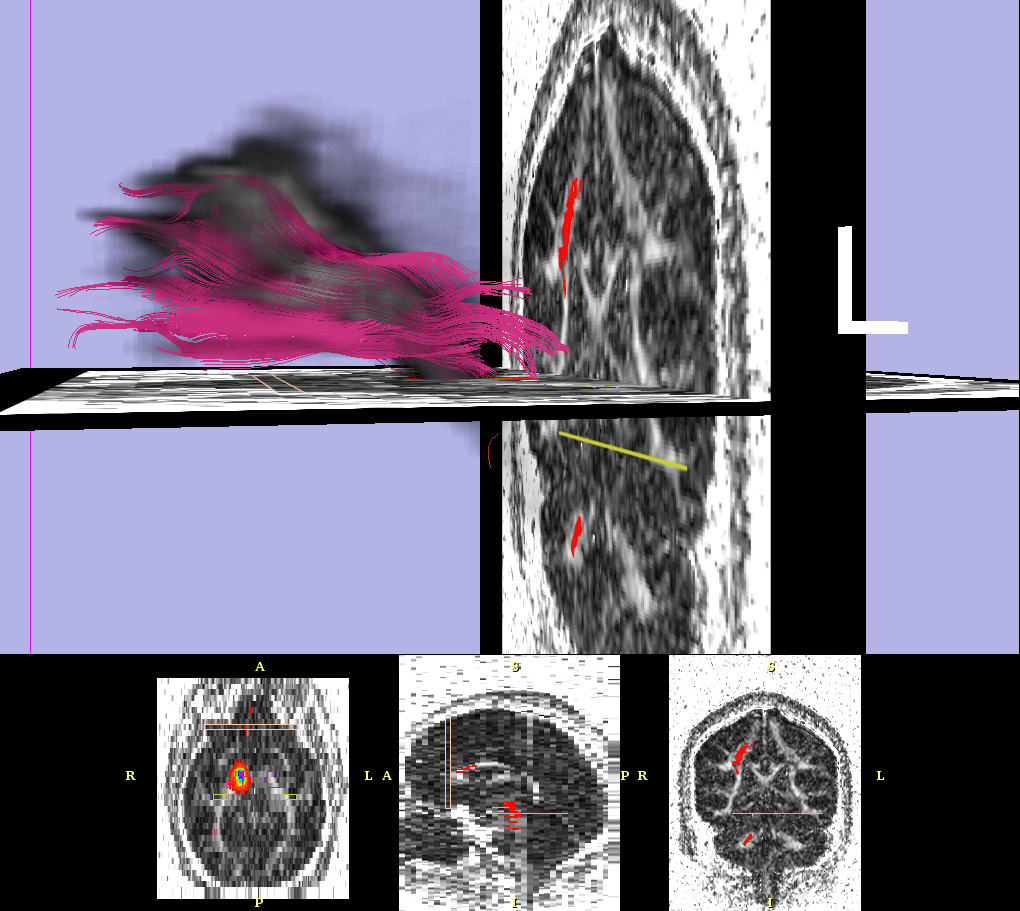
\includegraphics[width=0.5\linewidth]
	    {slicer-0015}
	  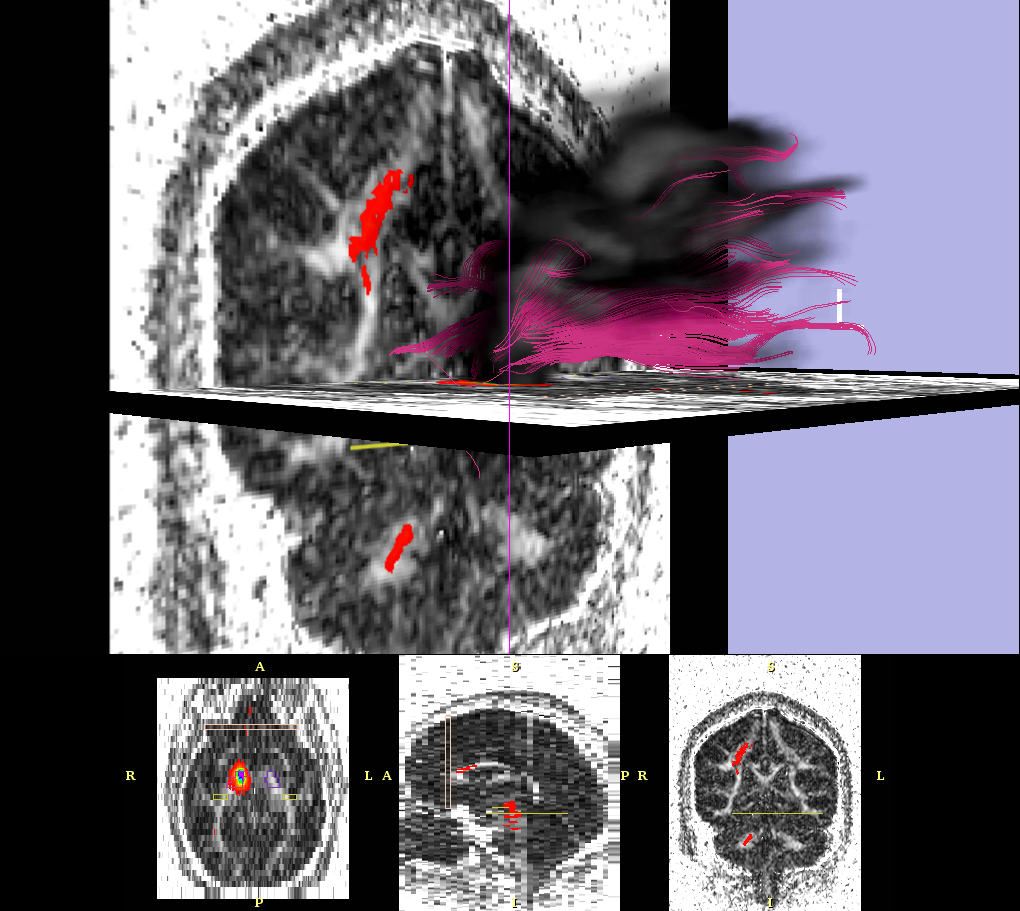
\includegraphics[width=0.5\linewidth]
	    {slicer-0017}
	}
	\caption{A comparison of streamlining and stochastic tractography results.  Results courtesy of Gudrun Rosenberger.}
\end{figure}

Figure \ref{fig:streamlinecomp:b} overlays a volume rendering of the connectivity map generated using stochastic tractography on the tracts generated using the streamlining method.  In this image the grey/black cloud is a 3D rendering of the connectivity map.  Although it is difficult to gauge the degree of connectivity in the volume rendering, it is clear that there exists regions which, according to stochastic tractography, have nonzero probability of connectivity but do not have streamline tracts passing through them.  Additionally, notice that in the region of the most inferior, or downward, streamline tracts, the stochastic tractography reports relatively weak connectivity.  The streamline method generates tracts in this improbable region because the anisotropy in this area is above the minimum threshold.  However since the stochastic tractography method takes into account the uncertainty in fiber direction, it determines that these tracts are much less likely to occur than a tract which is more superior, or upwards.

\begin{table} \label{tab:streamlinecomp}
  \center
  \begin{tabular}{cc}
    \hline & Mean Tract-Average FA\\
    \hline Stochastic Tractography & 0.4612\\
    Streamline Tractography & 0.36859\\
    \hline
  \end{tabular}
  \caption{Comparison of means of tract-averaged fractional anisotropy values under stochastic and streamlining methods.}
\end{table}

Finally, table \ref{tab:streamlinecomp} compares the mean of the distribution of tract-averaged fractional anisotropy values.  The stochastic tractography results may have a higher mean because tracts which pass through more anisotropic regions occur with greater frequency, weighing the mean tract-averaged fractional anisotropy value towards a higher value.



%show tracking in various regions, show correllation with anatomical figures
%show tracking with and without white matter posterior probability map

%show performance improvement with increasing threads
%show performance wrt increasing tract number.
